\documentclass[a4paper,11pt,UTF8]{article}
\usepackage{ctex}
\usepackage{amsmath,amsthm,amssymb,amsfonts}
\usepackage{amsmath}
\usepackage[a4paper]{geometry}
\usepackage{graphicx}
\usepackage{microtype}
\usepackage{siunitx}
\usepackage{booktabs}
\usepackage[colorlinks=false, pdfborder={0 0 0}]{hyperref}
\usepackage{cleveref}
\usepackage{esint} 
\usepackage{graphicx}
\usepackage{ragged2e}
\usepackage{pifont}
\usepackage{extarrows}
\usepackage{mathptmx}
\usepackage{float}
\usepackage{caption}
\captionsetup[figure]{name={Figure}}

\title{Microelectronics Circuit Analysis and Design Homework(12nd)}
\author{Yuejin Xie \quad U202210333}
\date{Oct 27th, 2023}
\begin{document}
\maketitle
11.35 The bias voltages of the diff-amp shown in Figure P11.35 are $V^+=5$V, $V^-=-5$V. The threshold voltage of each transistor is  $V_{TN}=0.4$V and assume $\lambda=0$. Let $K_{n3}=K_{n4}=0.20$ mA/V$^{2}$. The drain currents can be written as and $I_{D1}=K_{n1}\left(V_{GS1}-V_{TN}\right)^{2}$ and $I_{D2}=K_{n2}\left(V_{GS2}-V_{TN}\right)^{2}$.(a) Design the circuit  such that $I_Q=0.25$mA when $v_{1}=v_2=0$ (b) If $v_1= v_2= 0$ and $K_{n1}= K_{n2}= $ $ {0.120}$mA$/N^2,$ find $v_{O1}- v_{O2}$ when (i)$ R_{D1}=R_{D2}=15$k$\Omega$ (ii) $R_{D1}= 14.5$k$\Omega, R_{D2}= 15.5$k$\Omega$.(c) Repeat part (b)  for $K_{n1}= 0.125\mathrm{mA/V}^{2}$ and $K_{n2}= 0.115\mathrm{mA/V}^{2}.$
\begin{figure}[H]
	\centering
	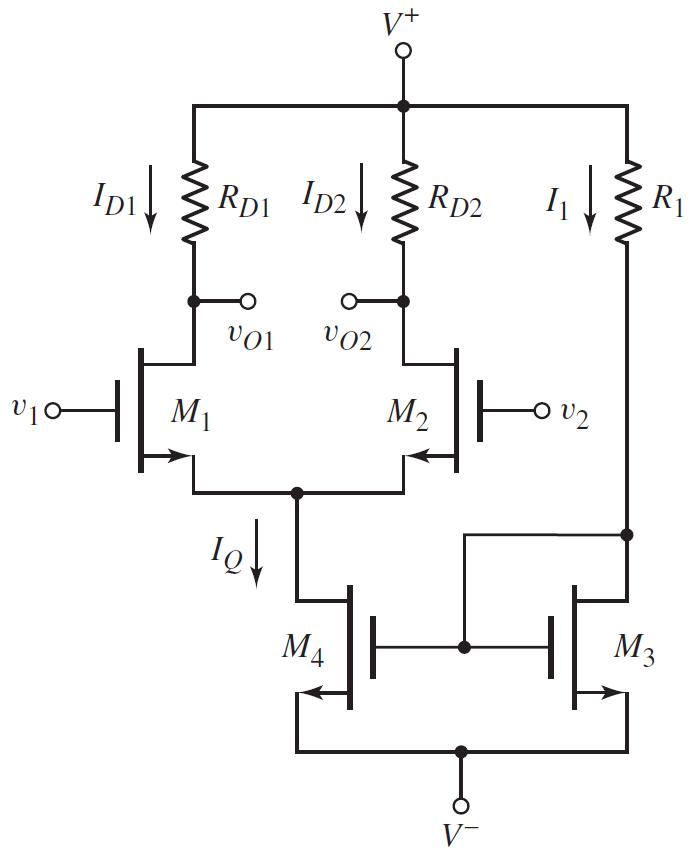
\includegraphics[width=0.5\textwidth]{11.35}
	\caption{Problem 11.35}
\end{figure}
\noindent Solution:

(a)$$
	I_{Q}=I_1=K_{n3}(V_{GS3}-V_{TN})^2\Rightarrow V_{GS3}=1.518\mathrm{V}
$$

Therefore:
$$
	R_1=\frac{V^+-V^-+V_{GS3}}{I_1}=33.9\mathrm{k\Omega}
$$

(b)$$
	v_{O1}=V^+-I_{D1}R_{D1},v_{O2}=V^+-I_{D2}R_{D2},I_{D1}=I_{D2}=\frac12I_Q
$$
$$
	\Rightarrow v_{O1}-v_{O2}=I_{D2}R_{D2}-I_{D1}R_{D1}
$$

(i)$ R_{D1}=R_{D2}=15$k$\Omega,v_{O1}-v_{O2}=0$

(ii) $R_{D1}= 14.5$k$\Omega, R_{D2}= 15.5$k$\Omega,v_{O1}-v_{O2}=0.125$V

(c)
$$\left\{\begin{aligned}
	&I_{Q}=I_{D1}+I_{D2}\\
	&I_{D1}=K_{n1}\left(V_{GS1}-V_{TN}\right)^{2}\\ &I_{D2}=K_{n2}\left(V_{GS2}-V_{TN}\right)^{2}
\end{aligned}\right.
\Rightarrow\begin{cases}
	I_{D1}=0.1302\mathrm{mA}\\
	I_{D2}=0.1198\mathrm{mA}
\end{cases}
$$

(i)$ R_{D1}=R_{D2}=15$k$\Omega,v_{O1}-v_{O2}=-0.156$V 

(ii) $R_{D1}= 14.5$k$\Omega, R_{D2}= 15.5$k$\Omega,v_{O1}-v_{O2}=0.031$V

11.47  Consider the circuit shown in Figure P11.47. Assume that $\lambda=0$ for $M_{1}$ and $M_{2}$. Also assume an ideal current source $I_{Q}$. Derive the expression for the one-sided differential mode gains  $A_{d1}= v_{o1}/v_d$ and $A_{d2}= v_{o2}/v_d, $ and the two-sided differential-mode gain $A_d=(v_{o2}-v_{o1})/v_d$ 
\begin{figure}[H]
	\centering
	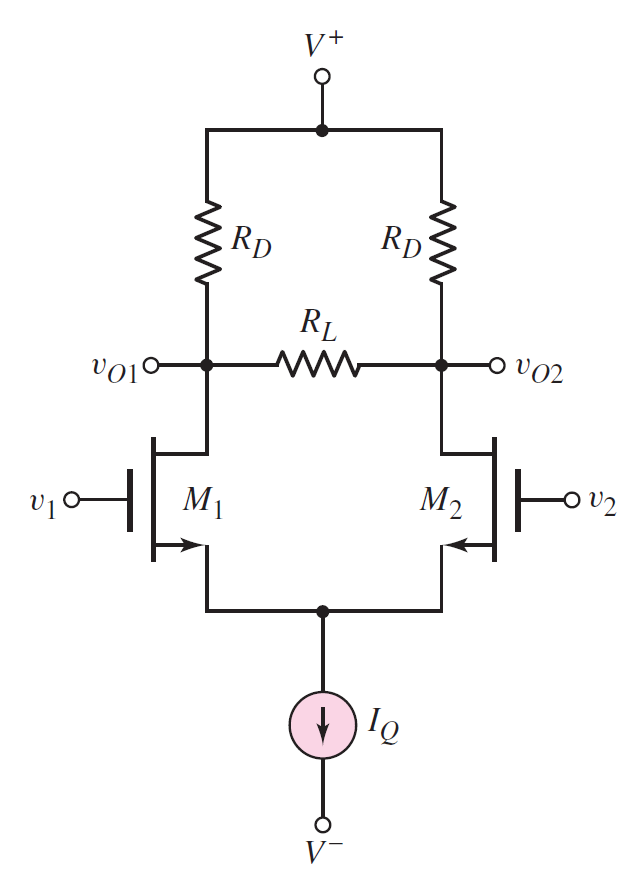
\includegraphics[width=0.5\textwidth]{11.47}
	\caption{Problem 11.47}
\end{figure}
\noindent Solution:

$$A_{d1}=-\frac12g_m(R_D||R_L),A_{d2}=\frac12g_m(R_D||R_L),A_d=g_m(R_d||\frac12R_L)$$

*D11.53  Figure P11.53 shows a two-stage cascade diff-amp with resistive loads. Power supply voltages of ±10 V are available. Assume transistor parameters of $V_{TN}=1$V, $k_n^{\prime}=60$ $\mu\mathrm{A/V^2}$, and $\lambda=0$. Design the circuit such that the two-sided differential-mode voltage gain is $A_{d1}=(v_{o2}-v_{o1})/(v_1-v_2)=20$ for the first stage, and that the one-sided differential-mode voltage gain is $A_{d2}=v_{o3}/(v_{o2}-v_{o1})=30$ for the second stage. The circuit is to be designed such that the maximum differential-mode voltage swing is obtained in each stage.
\begin{figure}[H]
	\centering
	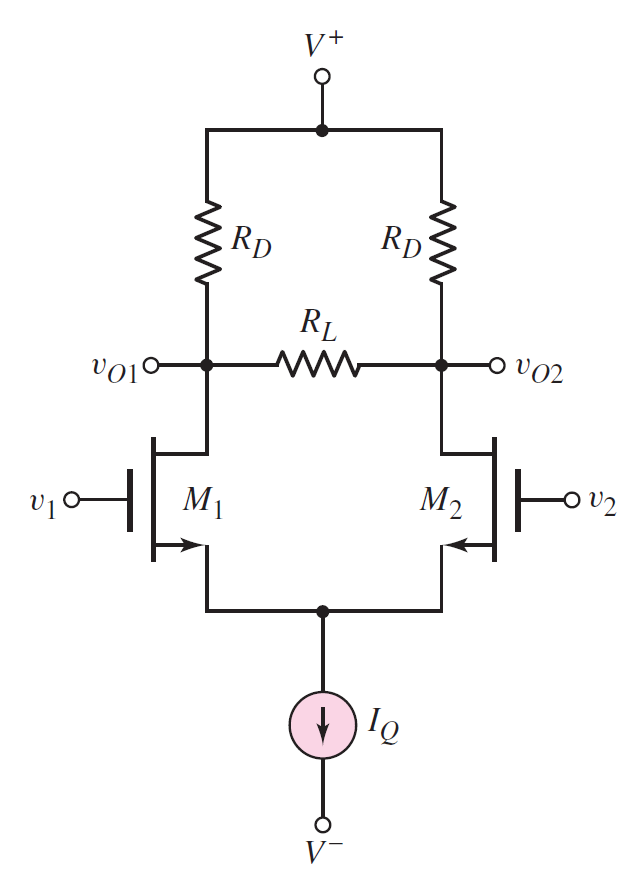
\includegraphics[width=0.5\textwidth]{11.47}
	\caption{Problem *D11.53}
\end{figure}
\noindent Solution:

$$ \\
	A_{d1}=\frac{\nu_{o2}-\nu_{o1}}{\nu_{1}-\nu_{2}}=g_{m1}R_{1}=\sqrt{2K_{n1}I_{Q1}}\cdot R_{1}=20 ,
	A_{d2}=\frac{\nu_{o3}}{\nu_{o2}-\nu_{o1}}=\frac{1}{2}g_{m3}R_{2}=\frac{1}{2}\sqrt{2K_{n3}I_{Q2}}\cdot R_{2}=30 
$$
$$
	\frac{I_{Q1}R_{1}}{2}=5V,\frac{I_{Q2}R_{2}}{2}=2.5V
	$$
$$
	{Let}I_{Q1}=I_{Q2}=0.1mA\Rightarrow R_{1}=100k\Omega,\quad R_{2}=50k\Omega
$$ 
$$
	2{\left({\frac{0.06}{2}}\right)}{\left({\frac{W}{L}}\right)}_{1}\left(0.1\right)={\left({\frac{20}{100}}\right)}^{2}\Rightarrow{\left({\frac{W}{L}}\right)}_{1}={\left({\frac{W}{L}}\right)}_{2}=6.67 
$$
$$
	2{\left({\frac{0.060}{2}}\right)}{\left({\frac{W}{L}}\right)}_{3}{\left(0.1\right)}={\left({\frac{2\left(30\right)}{50}}\right)}^{2}\Rightarrow{\left({\frac{W}{L}}\right)}_{3}={\left({\frac{W}{L}}\right)}_{4}=240
$$
\end{document}